\documentclass{standalone}

% ==== Essential Packages ====
\usepackage{tikz}
\usepackage{amsmath}
\usepackage{xcolor}
\usepackage{physics}
\usepackage{siunitx}
\usepackage{graphicx}
\usepackage{booktabs}
\usepackage{setspace}
\usepackage[font=small,labelfont=bf]{caption}
\usepackage[absolute,overlay]{textpos}
\usepackage{transparent}
\usepackage[subrefformat=parens,labelformat=parens]{subcaption}
\usepackage{shadowtext}
\usepackage{colortbl}
\usepackage[most]{tcolorbox}

% ==== TikZ Libraries ====
\usetikzlibrary{arrows.meta, decorations.pathreplacing, backgrounds, positioning, calc, shapes.geometric, decorations.pathmorphing}

% ==== Custom Colors ====
\definecolor{softyellow}{HTML}{F2D648}
\definecolor{dustyblue}{HTML}{9EB9D4}
\definecolor{berkeleyblue}{RGB}{0,50,98}
\definecolor{berkeleygold}{RGB}{253,181,21}
\definecolor{berkeleylight}{RGB}{198,217,241}
\definecolor{chalcogen}{RGB}{218,165,32}
\definecolor{metal}{RGB}{100,149,237}
\definecolor{tablegray}{gray}{0.95}
\definecolor{methodblue}{RGB}{100,120,180}
\definecolor{colgold}{RGB}{253,235,150} % very light gold tone

% ==== Custom tcolorbox ====
\newtcolorbox{rankingblock}[1]{
  colback=colgold,        % Background color
  colframe=berkeleyblue,  % Border color
  boxrule=0.4pt,
  arc=1mm,
  fontupper=\scriptsize,
  title=#1
}

\begin{document}

% Side-by-side TikZ figures using subfigure layout
\begin{center}
\begin{minipage}{0.48\linewidth}
\centering
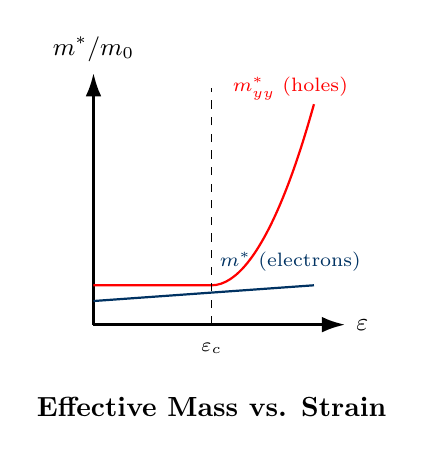
\begin{tikzpicture}[
  > = {Latex[length=3mm, width=2mm]},
  thick arrow/.style = {->, line width=1.2pt}
]
  \draw[thick arrow] (0,0) -- (3.2,0) node[right] {\small $\varepsilon$};
  \draw[thick arrow] (0,0) -- (0,3.2) node[above] {\small $m^*/m_0$};
  
  \draw[thick, red] (0,0.5) -- (1.5,0.5) parabola (2.8,2.8);
  \node[red] at (2.5,3) {\scriptsize $m^*_{yy}$ (holes)};
  
  \draw[thick, berkeleyblue] (0,0.3) -- (2.8,0.5);
  \node[berkeleyblue] at (2.5,0.8) {\scriptsize $m^*$ (electrons)};
  
  \draw[dashed] (1.5,0) -- (1.5,3);
  \node at (1.5,-0.3) {\scriptsize $\varepsilon_c$};
  
  \node[below] at (1.5,-0.8) {\textbf{Effective Mass vs. Strain}};
\end{tikzpicture}
\end{minipage}
\hfill
\begin{minipage}{0.48\linewidth}
\centering
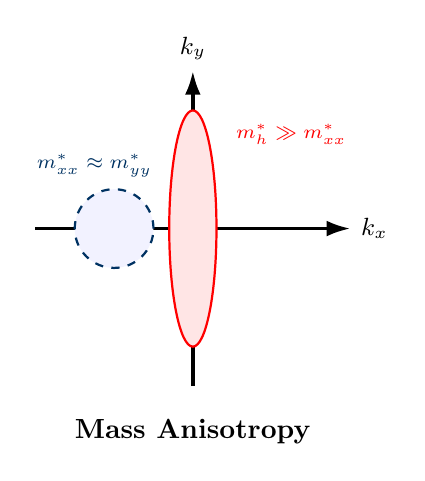
\begin{tikzpicture}[
  > = {Latex[length=3mm, width=2mm]},
  thick arrow/.style = {->, line width=1.2pt}
]
  \draw[thick arrow] (-2,0) -- (2,0) node[right] {\small $k_x$};
  \draw[thick arrow] (0,-2) -- (0,2) node[above] {\small $k_y$};
  
  \draw[thick, red, fill=red!10] (0,0) ellipse (0.3 and 1.5);
  \node[red] at (1.25,1.2) {\scriptsize $m^*_h \gg m^*_{xx}$};
  
  \draw[thick, berkeleyblue, fill=blue!5, dashed] (-1,0) circle (0.5);
  \node[berkeleyblue] at (-1.25,0.8) {\scriptsize $m^*_{xx} \approx m^*_{yy}$};
  
  \node[below] at (0,-2.3) {\textbf{Mass Anisotropy}};
\end{tikzpicture}
\end{minipage}
\end{center}

\end{document}
